\section{Statistic Class Reference}
\label{classStatistic}\index{Statistic@{Statistic}}
{\tt \#include $<$stats.h$>$}

Inheritance diagram for Statistic:\nopagebreak
\begin{figure}[H]
\begin{center}
\leavevmode
\includegraphics[height=400pt]{classStatistic__inherit__graph}
\end{center}
\end{figure}
Collaboration diagram for Statistic:\nopagebreak
\begin{figure}[H]
\begin{center}
\leavevmode
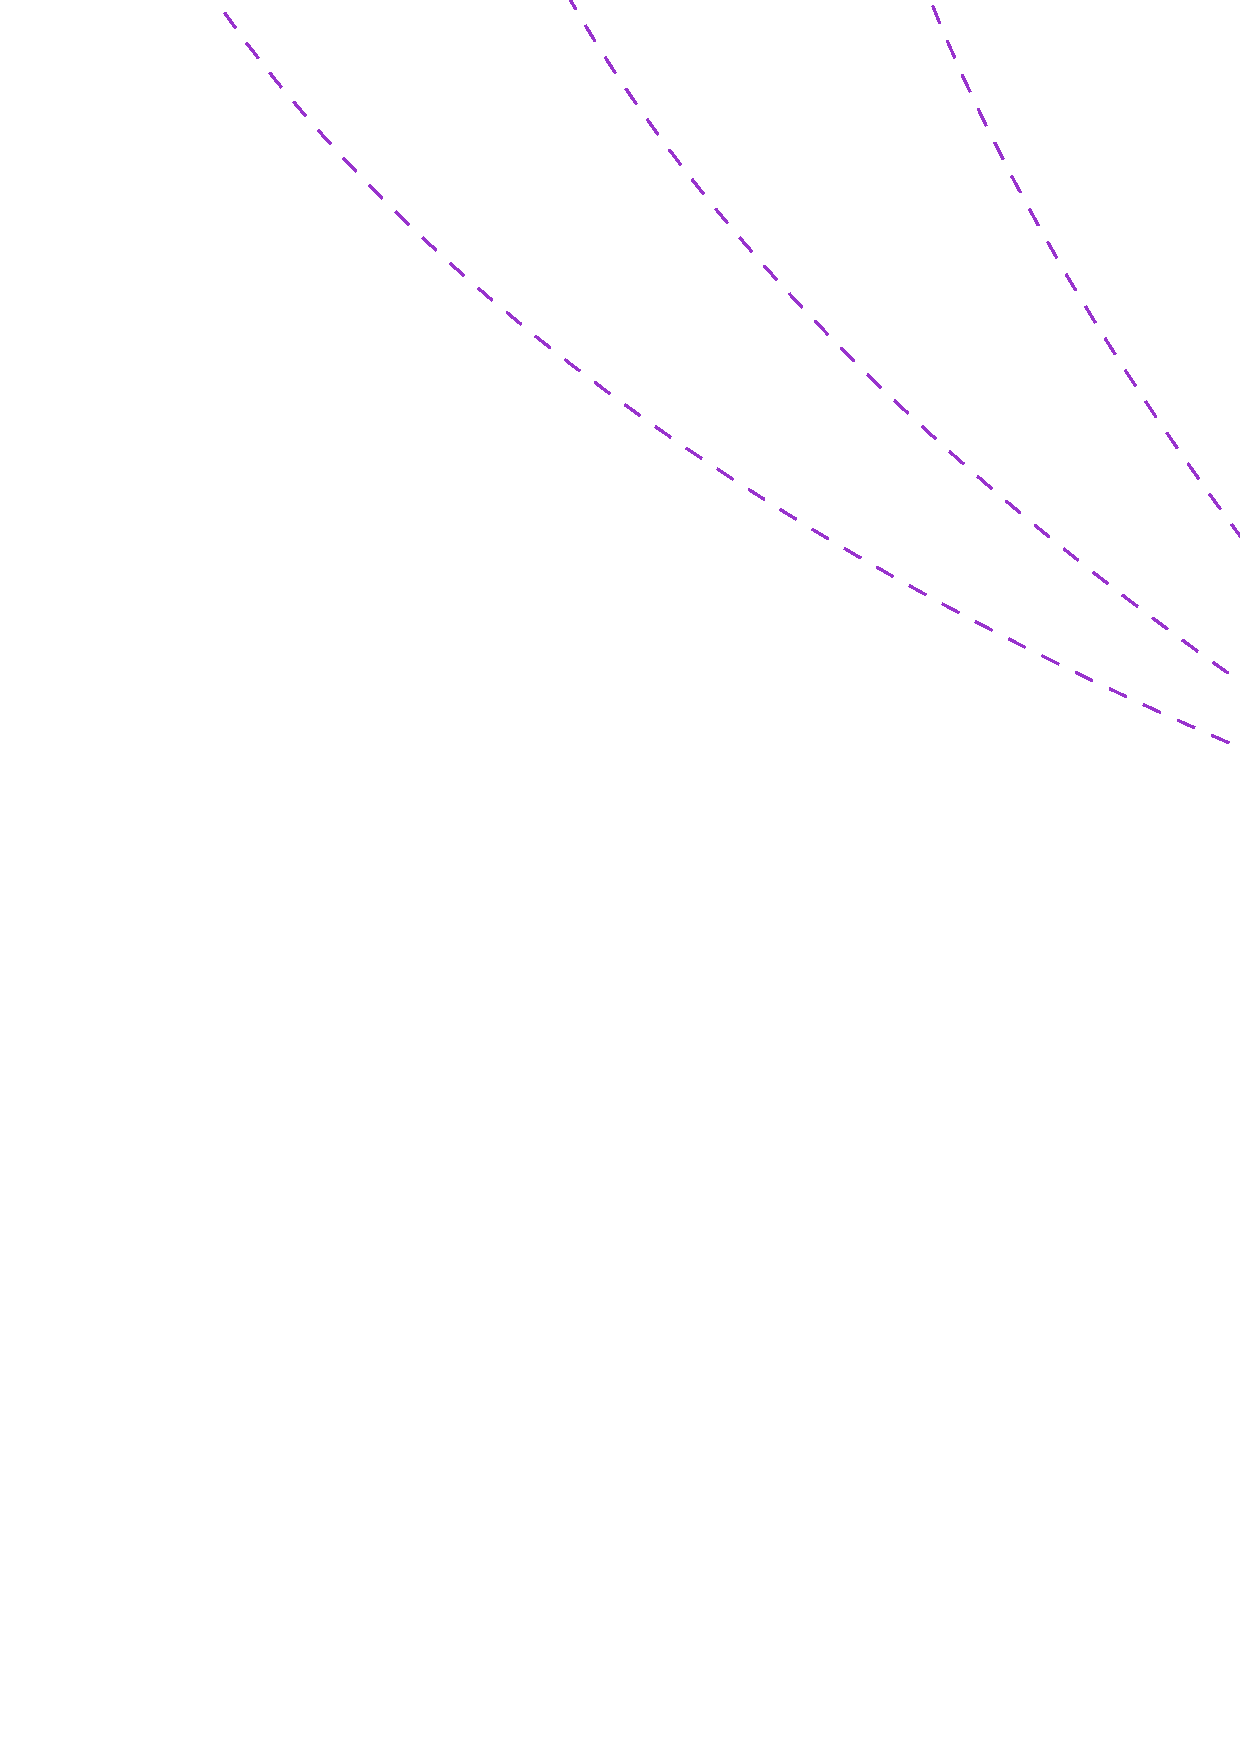
\includegraphics[width=400pt]{classStatistic__coll__graph}
\end{center}
\end{figure}
\subsection*{Public Member Functions}
\begin{CompactItemize}
\item 
void {\bf InitStats} ()
\item 
void {\bf CollectStatsPerRequest} ({\bf Request} $\ast$req)
\item 
void {\bf CalculateAggregateStats} ()
\item 
string {\bf PrintAggregateStats} ({\bf uint} n)
\item 
void {\bf CollectStatsPerCycle} ()
\end{CompactItemize}
\subsection*{Public Attributes}
\begin{CompactItemize}
\item 
{\bf Component} $\ast$ {\bf mc}
\item 
{\bf Component} $\ast$ {\bf pwr}
\item 
vector$<$ double $>$ {\bf avgLatPerBank}
\item 
vector$<$ {\bf ullint} $>$ {\bf latPerBank}
\item 
vector$<$ {\bf ullint} $>$ {\bf reqPerBank}
\item 
vector$<$ {\bf ullint} $>$ {\bf hitsPerBank}
\item 
vector$<$ {\bf ullint} $>$ {\bf throttlePerBank}
\item 
vector$<$ double $>$ {\bf avgThrottlePerBank}
\item 
vector$<$ double $>$ {\bf hitRatePerBank}
\item 
vector$<$ vector$<$ double $>$ $>$ {\bf avgLatPerThreadPerBank}
\item 
vector$<$ vector$<$ {\bf ullint} $>$ $>$ {\bf latPerThreadPerBank}
\item 
vector$<$ vector$<$ {\bf ullint} $>$ $>$ {\bf reqPerThreadPerBank}
\item 
vector$<$ vector$<$ {\bf ullint} $>$ $>$ {\bf hitsPerThreadPerBank}
\item 
vector$<$ vector$<$ {\bf ullint} $>$ $>$ {\bf throttlePerThreadPerBank}
\item 
vector$<$ vector$<$ double $>$ $>$ {\bf avgThrottlePerThreadPerBank}
\item 
vector$<$ vector$<$ double $>$ $>$ {\bf hitRatePerThreadPerBank}
\item 
vector$<$ vector$<$ {\bf ullint} $>$ $>$ {\bf TotalFrontSideTimePerThreadPerBank}
\item 
vector$<$ vector$<$ {\bf ullint} $>$ $>$ {\bf TotalQueueDelayPerThreadPerBank}
\item 
vector$<$ vector$<$ {\bf ullint} $>$ $>$ {\bf TotalCBufDelayPerThreadPerBank}
\item 
vector$<$ vector$<$ {\bf ullint} $>$ $>$ {\bf TotalBusMemDelayPerThreadPerBank}
\item 
vector$<$ vector$<$ vector$<$ {\bf ullint} $>$ $>$ $>$ {\bf rbufferOccupancy}
\item 
vector$<$ vector$<$ vector$<$ {\bf ullint} $>$ $>$ $>$ {\bf emptyCycles}
\item 
vector$<$ vector$<$ vector$<$ float $>$ $>$ $>$ {\bf rbufferOccupancyRatio}
\item 
vector$<$ {\bf ullint} $>$ {\bf TotalFrontSideTimePerBank}
\item 
vector$<$ {\bf ullint} $>$ {\bf TotalQueueDelayPerBank}
\item 
vector$<$ {\bf ullint} $>$ {\bf TotalCBufDelayPerBank}
\item 
vector$<$ {\bf ullint} $>$ {\bf TotalBusMemDelayPerBank}
\item 
vector$<$ float $>$ {\bf avgFrontSideTimePerBank}
\item 
vector$<$ float $>$ {\bf avgQueueDelayPerBank}
\item 
vector$<$ float $>$ {\bf avgCBufDelayPerBank}
\item 
vector$<$ float $>$ {\bf avgBusMemDelayPerBank}
\item 
bool $\ast$ {\bf doneOnce}
\item 
vector$<$ double $>$ {\bf avgLatPerThread}
\item 
vector$<$ {\bf ullint} $>$ {\bf latPerThread}
\item 
vector$<$ {\bf ullint} $>$ {\bf reqPerThread}
\item 
vector$<$ {\bf ullint} $>$ {\bf hitsPerThread}
\item 
vector$<$ {\bf ullint} $>$ {\bf throttlePerThread}
\item 
vector$<$ double $>$ {\bf avgThrottlePerThread}
\item 
vector$<$ double $>$ {\bf hitRatePerThread}
\item 
vector$<$ float $>$ {\bf BLPPerThread}
\item 
vector$<$ {\bf ullint} $>$ {\bf TotalFrontSideTimePerThread}
\item 
vector$<$ {\bf ullint} $>$ {\bf TotalQueueDelayPerThread}
\item 
vector$<$ {\bf ullint} $>$ {\bf TotalCBufDelayPerThread}
\item 
vector$<$ {\bf ullint} $>$ {\bf TotalBusMemDelayPerThread}
\item 
vector$<$ float $>$ {\bf avgFrontSideTimePerThread}
\item 
vector$<$ float $>$ {\bf avgQueueDelayPerThread}
\item 
vector$<$ float $>$ {\bf avgCBufDelayPerThread}
\item 
vector$<$ float $>$ {\bf avgBusMemDelayPerThread}
\item 
vector$<$ vector$<$ vector$<$ {\bf ullint} $>$ $>$ $>$ {\bf bufferFullCycles}
\item 
float {\bf BNK\_\-PRE}
\item 
float {\bf CLK\_\-LO\_\-PRE}
\item 
float {\bf CLK\_\-LO\_\-ACT}
\item 
float {\bf PH}
\item 
float {\bf RDsch}
\item 
float {\bf WRsch}
\item 
float {\bf termRDsch}
\item 
float {\bf termWRsch}
\item 
float {\bf RRDsch}
\end{CompactItemize}


\subsection{Detailed Description}


Definition at line 29 of file memctrl/stats.h.

\subsection{Member Function Documentation}
\index{Statistic@{Statistic}!CalculateAggregateStats@{CalculateAggregateStats}}
\index{CalculateAggregateStats@{CalculateAggregateStats}!Statistic@{Statistic}}
\subsubsection[{CalculateAggregateStats}]{\setlength{\rightskip}{0pt plus 5cm}void Statistic::CalculateAggregateStats ()}\label{classStatistic_833f4ab2c90268e5abf2a5b2e9906a31}




Definition at line 334 of file stats.cc.

References avgBusMemDelayPerBank, avgBusMemDelayPerThread, avgCBufDelayPerBank, avgCBufDelayPerThread, avgFrontSideTimePerBank, avgFrontSideTimePerThread, avgLatPerBank, avgLatPerThread, avgLatPerThreadPerBank, avgQueueDelayPerBank, avgQueueDelayPerThread, avgThrottlePerBank, avgThrottlePerThread, avgThrottlePerThreadPerBank, BL, BNK\_\-PRE, bufferFullCycles, CLK\_\-LO\_\-ACT, CLK\_\-LO\_\-PRE, hitRatePerBank, hitRatePerThread, hitsPerBank, hitsPerThread, hitsPerThreadPerBank, latPerBank, latPerThread, latPerThreadPerBank, mc, NO\_\-OF\_\-BANKS, NO\_\-OF\_\-CHANNELS, NO\_\-OF\_\-RANKS, NO\_\-OF\_\-THREADS, Simulator::Now(), PH, pwr, rbufferOccupancyRatio, RDsch, reqPerBank, reqPerThread, reqPerThreadPerBank, RRDsch, SysClk, termRDsch, termWRsch, throttlePerBank, throttlePerThread, throttlePerThreadPerBank, TotalBusMemDelayPerBank, TotalBusMemDelayPerThread, TotalBusMemDelayPerThreadPerBank, TotalCBufDelayPerBank, TotalCBufDelayPerThread, TotalCBufDelayPerThreadPerBank, TotalFrontSideTimePerBank, TotalFrontSideTimePerThread, TotalFrontSideTimePerThreadPerBank, TotalQueueDelayPerBank, TotalQueueDelayPerThread, TotalQueueDelayPerThreadPerBank, and WRsch.

Referenced by main().

Here is the caller graph for this function:\nopagebreak
\begin{figure}[H]
\begin{center}
\leavevmode
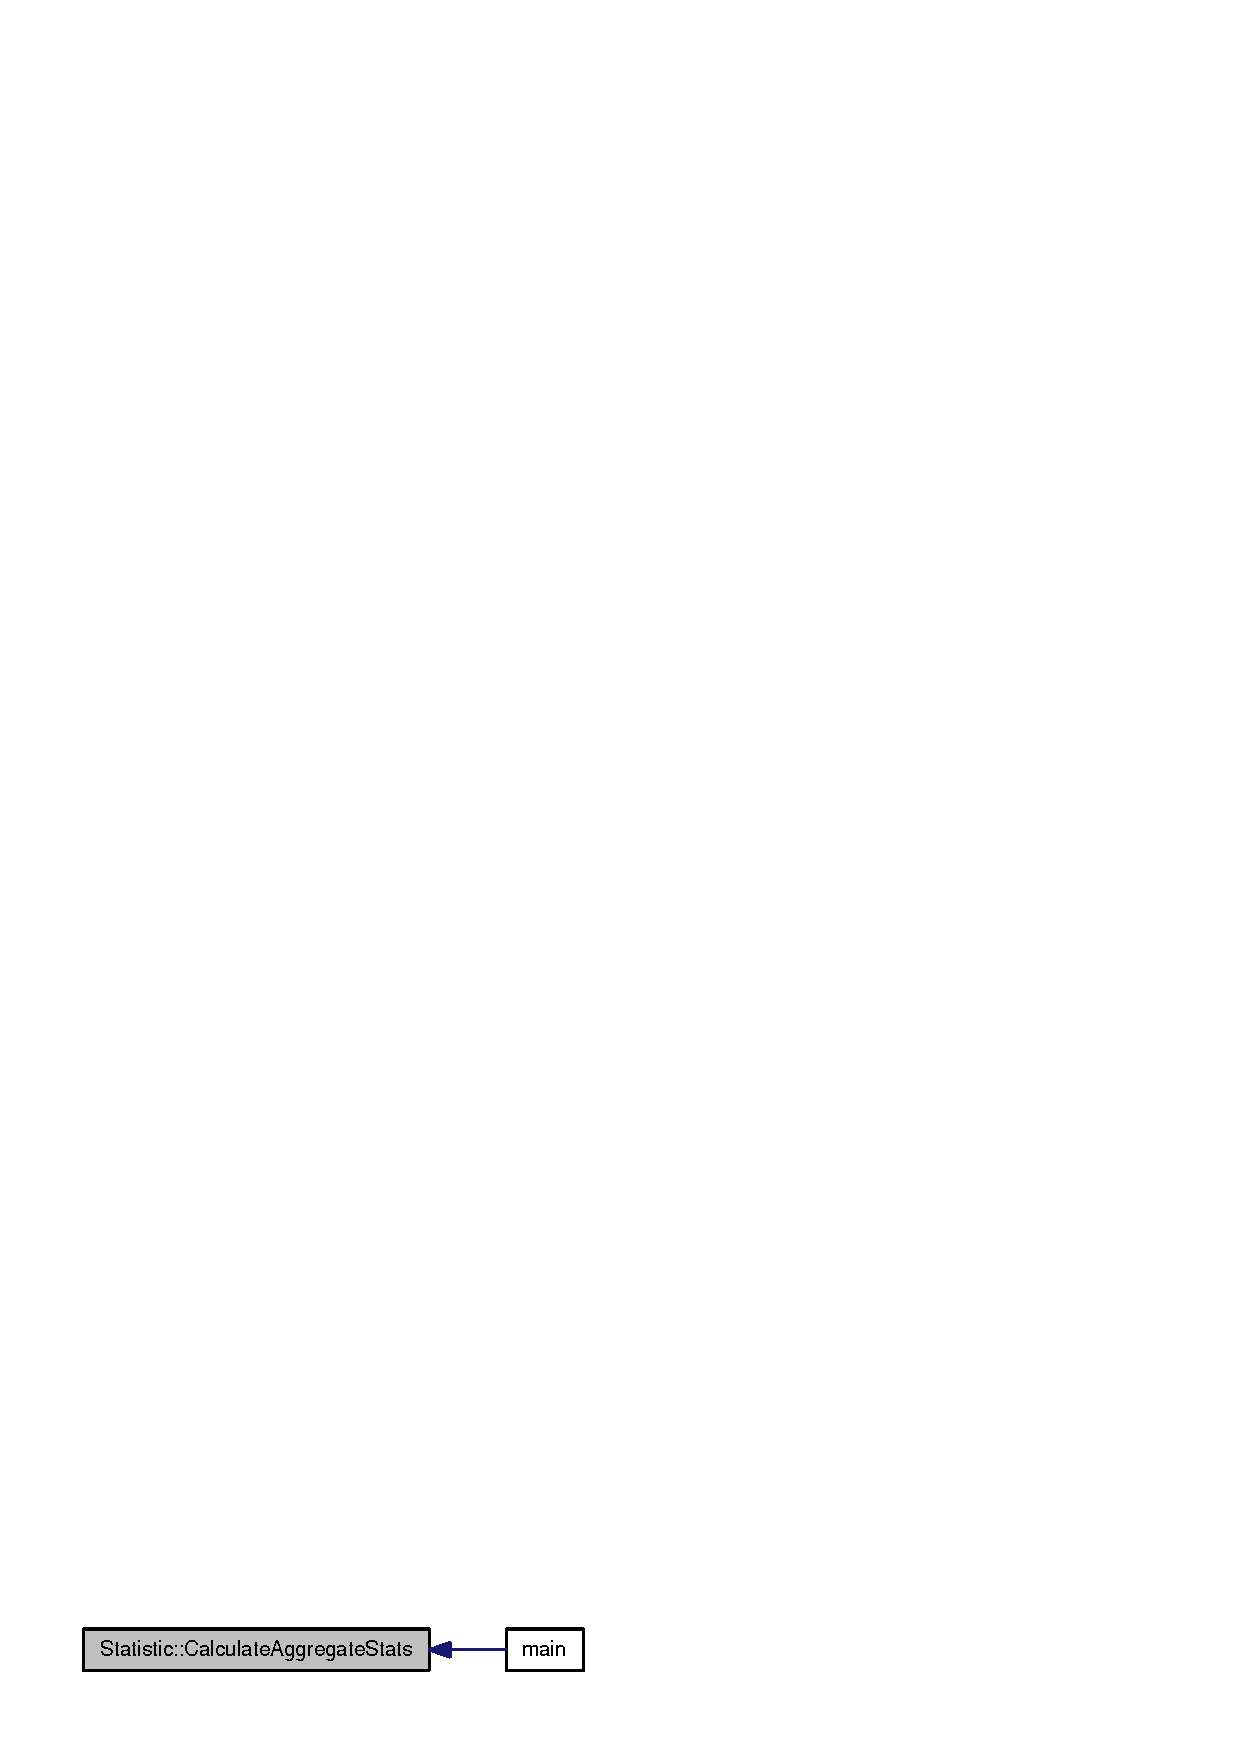
\includegraphics[width=142pt]{classStatistic_833f4ab2c90268e5abf2a5b2e9906a31_icgraph}
\end{center}
\end{figure}
\index{Statistic@{Statistic}!CollectStatsPerCycle@{CollectStatsPerCycle}}
\index{CollectStatsPerCycle@{CollectStatsPerCycle}!Statistic@{Statistic}}
\subsubsection[{CollectStatsPerCycle}]{\setlength{\rightskip}{0pt plus 5cm}void Statistic::CollectStatsPerCycle ()}\label{classStatistic_236ec4d09c07aeaf8311061cfe837a08}




Definition at line 135 of file stats.cc.

References NO\_\-OF\_\-BUFFERS, NO\_\-OF\_\-CHANNELS, and NO\_\-OF\_\-RANKS.

Referenced by main().

Here is the caller graph for this function:\nopagebreak
\begin{figure}[H]
\begin{center}
\leavevmode
\includegraphics[width=135pt]{classStatistic_236ec4d09c07aeaf8311061cfe837a08_icgraph}
\end{center}
\end{figure}
\index{Statistic@{Statistic}!CollectStatsPerRequest@{CollectStatsPerRequest}}
\index{CollectStatsPerRequest@{CollectStatsPerRequest}!Statistic@{Statistic}}
\subsubsection[{CollectStatsPerRequest}]{\setlength{\rightskip}{0pt plus 5cm}void Statistic::CollectStatsPerRequest ({\bf Request} $\ast$ {\em req})}\label{classStatistic_b9e517fce7d9ae39a851fd4eb8ec6d8e}




Definition at line 89 of file stats.cc.

References Request::address, Request::arrivalTime, avgLatPerThreadPerBank, avgThrottlePerThreadPerBank, Request::bankNo, Request::busInsertionTime, Request::cbufferInsertionTime, hitRatePerThreadPerBank, hitsPerThreadPerBank, latPerThreadPerBank, mc, Simulator::Now(), OPEN, Request::rbufferInsertionTime, reqPerThreadPerBank, Request::retireTime, Request::status, Request::threadId, Request::throttleTime, TotalBusMemDelayPerThreadPerBank, TotalCBufDelayPerThreadPerBank, TotalFrontSideTimePerThreadPerBank, and TotalQueueDelayPerThreadPerBank.\index{Statistic@{Statistic}!InitStats@{InitStats}}
\index{InitStats@{InitStats}!Statistic@{Statistic}}
\subsubsection[{InitStats}]{\setlength{\rightskip}{0pt plus 5cm}void Statistic::InitStats ()}\label{classStatistic_fabb153ded71e9865b72ad0da907de0f}




Definition at line 152 of file stats.cc.

References avgBusMemDelayPerBank, avgBusMemDelayPerThread, avgCBufDelayPerBank, avgCBufDelayPerThread, avgFrontSideTimePerBank, avgFrontSideTimePerThread, avgLatPerBank, avgLatPerThread, avgLatPerThreadPerBank, avgQueueDelayPerBank, avgQueueDelayPerThread, avgThrottlePerBank, avgThrottlePerThread, avgThrottlePerThreadPerBank, BLPPerThread, BNK\_\-PRE, bufferFullCycles, CLK\_\-LO\_\-ACT, CLK\_\-LO\_\-PRE, emptyCycles, hitRatePerBank, hitRatePerThread, hitRatePerThreadPerBank, hitsPerBank, hitsPerThread, hitsPerThreadPerBank, latPerBank, latPerThread, latPerThreadPerBank, NO\_\-OF\_\-BANKS, NO\_\-OF\_\-BUFFERS, NO\_\-OF\_\-CHANNELS, NO\_\-OF\_\-RANKS, NO\_\-OF\_\-THREADS, PH, pwr, rbufferOccupancy, rbufferOccupancyRatio, RDsch, reqPerBank, reqPerThread, reqPerThreadPerBank, termRDsch, termWRsch, throttlePerBank, throttlePerThread, throttlePerThreadPerBank, TotalBusMemDelayPerBank, TotalBusMemDelayPerThread, TotalBusMemDelayPerThreadPerBank, TotalCBufDelayPerBank, TotalCBufDelayPerThread, TotalCBufDelayPerThreadPerBank, TotalFrontSideTimePerBank, TotalFrontSideTimePerThread, TotalFrontSideTimePerThreadPerBank, TotalQueueDelayPerBank, TotalQueueDelayPerThread, TotalQueueDelayPerThreadPerBank, and WRsch.

Referenced by MC::Init().

Here is the caller graph for this function:\nopagebreak
\begin{figure}[H]
\begin{center}
\leavevmode
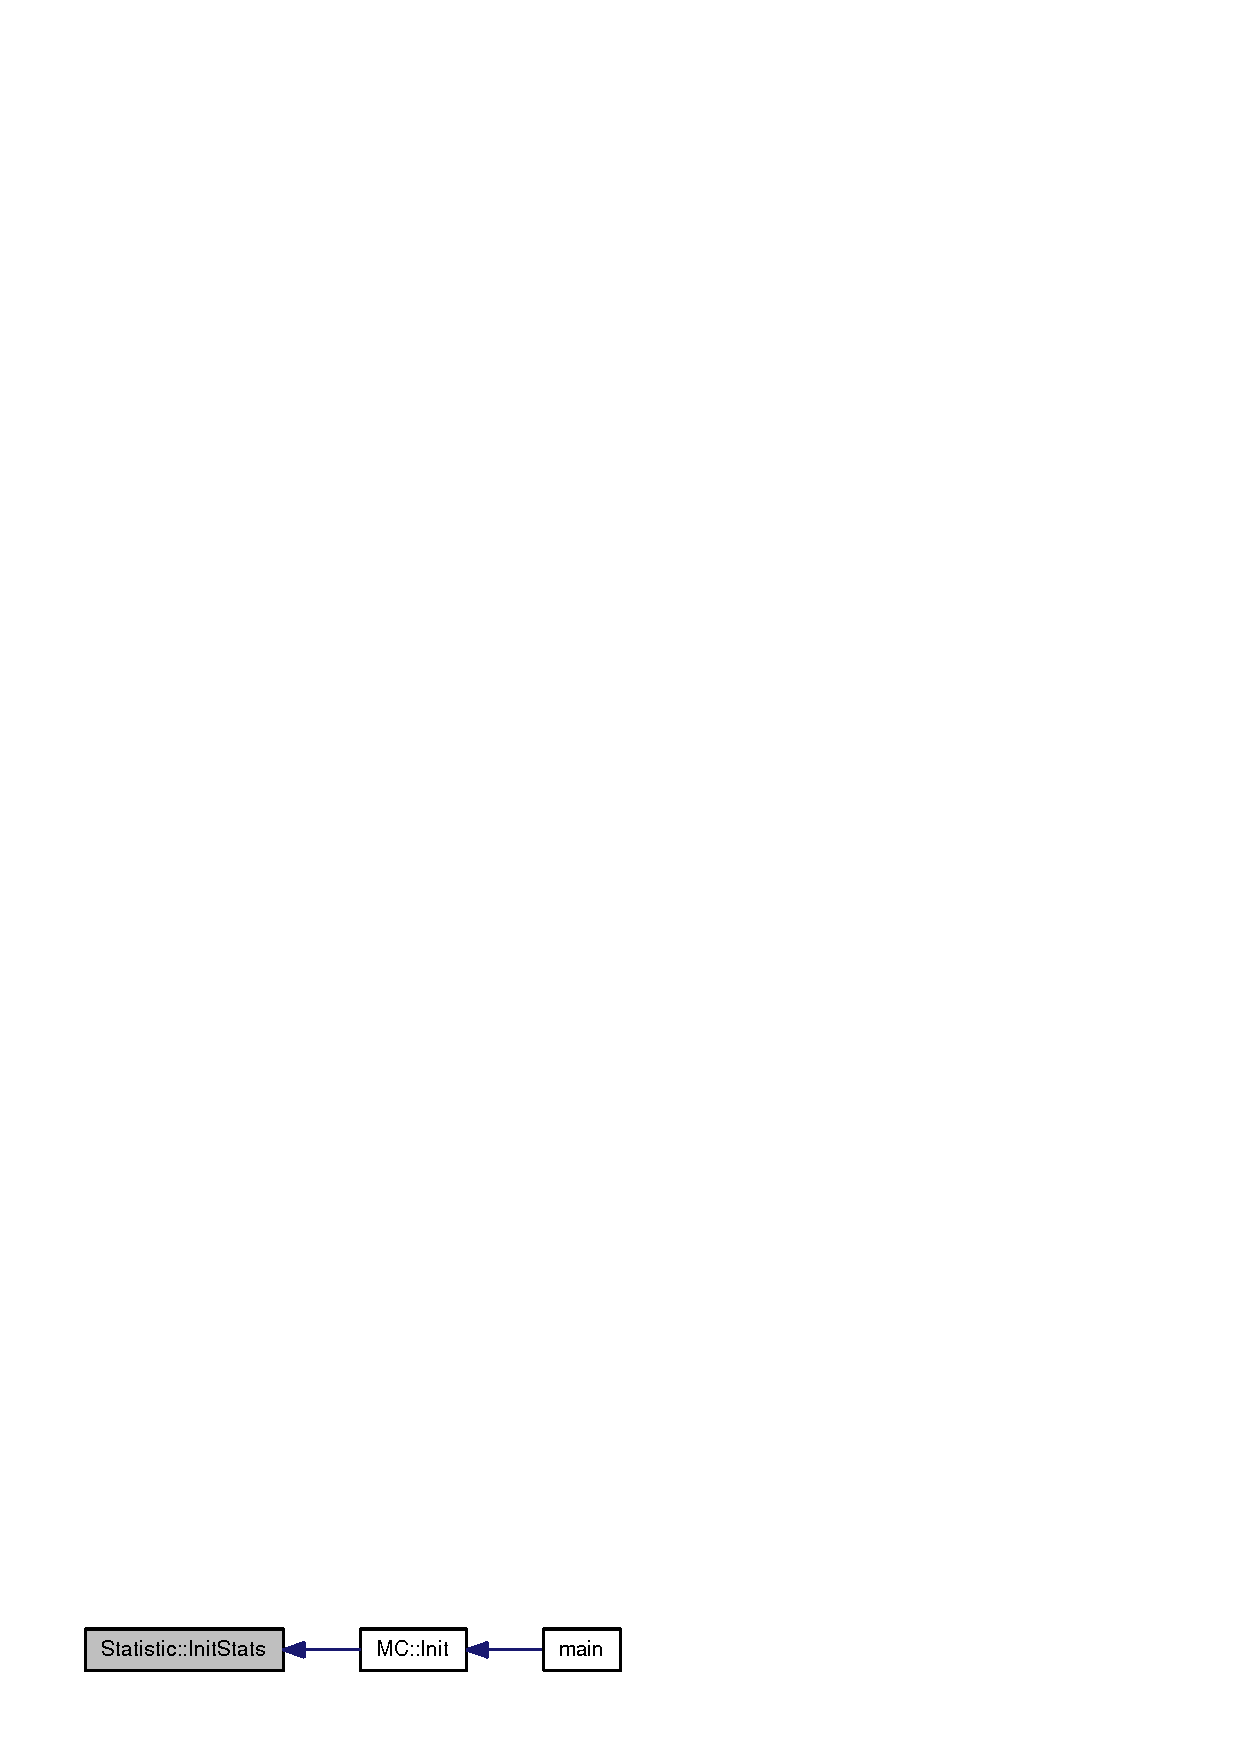
\includegraphics[width=151pt]{classStatistic_fabb153ded71e9865b72ad0da907de0f_icgraph}
\end{center}
\end{figure}
\index{Statistic@{Statistic}!PrintAggregateStats@{PrintAggregateStats}}
\index{PrintAggregateStats@{PrintAggregateStats}!Statistic@{Statistic}}
\subsubsection[{PrintAggregateStats}]{\setlength{\rightskip}{0pt plus 5cm}string Statistic::PrintAggregateStats ({\bf uint} {\em n})}\label{classStatistic_fba2d32119e3a6da2f56aaee19944cf6}




Definition at line 435 of file stats.cc.

References avgBusMemDelayPerBank, avgBusMemDelayPerThread, avgCBufDelayPerBank, avgCBufDelayPerThread, avgFrontSideTimePerBank, avgFrontSideTimePerThread, avgLatPerBank, avgLatPerThread, avgQueueDelayPerBank, avgQueueDelayPerThread, bufferFullCycles, hitRatePerBank, hitRatePerThread, hitsPerBank, hitsPerThread, mc, NO\_\-OF\_\-BANKS, NO\_\-OF\_\-BUFFERS, NO\_\-OF\_\-CHANNELS, NO\_\-OF\_\-RANKS, NO\_\-OF\_\-THREADS, Simulator::Now(), PH, pwr, rbufferOccupancyRatio, RDsch, reqPerBank, reqPerThread, and WRsch.

Referenced by main().

Here is the caller graph for this function:\nopagebreak
\begin{figure}[H]
\begin{center}
\leavevmode
\includegraphics[width=132pt]{classStatistic_fba2d32119e3a6da2f56aaee19944cf6_icgraph}
\end{center}
\end{figure}


\subsection{Member Data Documentation}
\index{Statistic@{Statistic}!avgBusMemDelayPerBank@{avgBusMemDelayPerBank}}
\index{avgBusMemDelayPerBank@{avgBusMemDelayPerBank}!Statistic@{Statistic}}
\subsubsection[{avgBusMemDelayPerBank}]{\setlength{\rightskip}{0pt plus 5cm}vector$<$float$>$ {\bf Statistic::avgBusMemDelayPerBank}}\label{classStatistic_51eed213cdd1ed75e43d63a17e12edd9}




Definition at line 72 of file memctrl/stats.h.

Referenced by CalculateAggregateStats(), InitStats(), and PrintAggregateStats().\index{Statistic@{Statistic}!avgBusMemDelayPerThread@{avgBusMemDelayPerThread}}
\index{avgBusMemDelayPerThread@{avgBusMemDelayPerThread}!Statistic@{Statistic}}
\subsubsection[{avgBusMemDelayPerThread}]{\setlength{\rightskip}{0pt plus 5cm}vector$<$float$>$ {\bf Statistic::avgBusMemDelayPerThread}}\label{classStatistic_32222891516aea41f7812234f911b39b}




Definition at line 98 of file memctrl/stats.h.

Referenced by CalculateAggregateStats(), InitStats(), and PrintAggregateStats().\index{Statistic@{Statistic}!avgCBufDelayPerBank@{avgCBufDelayPerBank}}
\index{avgCBufDelayPerBank@{avgCBufDelayPerBank}!Statistic@{Statistic}}
\subsubsection[{avgCBufDelayPerBank}]{\setlength{\rightskip}{0pt plus 5cm}vector$<$float$>$ {\bf Statistic::avgCBufDelayPerBank}}\label{classStatistic_b741691627211b72698a41d646aaaad1}




Definition at line 71 of file memctrl/stats.h.

Referenced by CalculateAggregateStats(), InitStats(), and PrintAggregateStats().\index{Statistic@{Statistic}!avgCBufDelayPerThread@{avgCBufDelayPerThread}}
\index{avgCBufDelayPerThread@{avgCBufDelayPerThread}!Statistic@{Statistic}}
\subsubsection[{avgCBufDelayPerThread}]{\setlength{\rightskip}{0pt plus 5cm}vector$<$float$>$ {\bf Statistic::avgCBufDelayPerThread}}\label{classStatistic_1dd806919a827b7c65c9ac62b5bf5e39}




Definition at line 97 of file memctrl/stats.h.

Referenced by CalculateAggregateStats(), InitStats(), and PrintAggregateStats().\index{Statistic@{Statistic}!avgFrontSideTimePerBank@{avgFrontSideTimePerBank}}
\index{avgFrontSideTimePerBank@{avgFrontSideTimePerBank}!Statistic@{Statistic}}
\subsubsection[{avgFrontSideTimePerBank}]{\setlength{\rightskip}{0pt plus 5cm}vector$<$float$>$ {\bf Statistic::avgFrontSideTimePerBank}}\label{classStatistic_1726ccf8d19f4e5bd79ea8427e92c311}




Definition at line 69 of file memctrl/stats.h.

Referenced by CalculateAggregateStats(), InitStats(), and PrintAggregateStats().\index{Statistic@{Statistic}!avgFrontSideTimePerThread@{avgFrontSideTimePerThread}}
\index{avgFrontSideTimePerThread@{avgFrontSideTimePerThread}!Statistic@{Statistic}}
\subsubsection[{avgFrontSideTimePerThread}]{\setlength{\rightskip}{0pt plus 5cm}vector$<$float$>$ {\bf Statistic::avgFrontSideTimePerThread}}\label{classStatistic_9019404110219ab38c24306e55cf14d0}




Definition at line 95 of file memctrl/stats.h.

Referenced by CalculateAggregateStats(), InitStats(), and PrintAggregateStats().\index{Statistic@{Statistic}!avgLatPerBank@{avgLatPerBank}}
\index{avgLatPerBank@{avgLatPerBank}!Statistic@{Statistic}}
\subsubsection[{avgLatPerBank}]{\setlength{\rightskip}{0pt plus 5cm}vector$<$double$>$ {\bf Statistic::avgLatPerBank}}\label{classStatistic_491c14bf3f158a4dca4e7f71640d25af}




Definition at line 38 of file memctrl/stats.h.

Referenced by CalculateAggregateStats(), InitStats(), and PrintAggregateStats().\index{Statistic@{Statistic}!avgLatPerThread@{avgLatPerThread}}
\index{avgLatPerThread@{avgLatPerThread}!Statistic@{Statistic}}
\subsubsection[{avgLatPerThread}]{\setlength{\rightskip}{0pt plus 5cm}vector$<$double$>$ {\bf Statistic::avgLatPerThread}}\label{classStatistic_7a6f92c59ce5d33f3c4a3a9913a708d5}




Definition at line 81 of file memctrl/stats.h.

Referenced by CalculateAggregateStats(), InitStats(), and PrintAggregateStats().\index{Statistic@{Statistic}!avgLatPerThreadPerBank@{avgLatPerThreadPerBank}}
\index{avgLatPerThreadPerBank@{avgLatPerThreadPerBank}!Statistic@{Statistic}}
\subsubsection[{avgLatPerThreadPerBank}]{\setlength{\rightskip}{0pt plus 5cm}vector$<$ vector$<$double$>$ $>$ {\bf Statistic::avgLatPerThreadPerBank}}\label{classStatistic_fdf7d59fa40a44cfe10fdaa54e295e68}




Definition at line 46 of file memctrl/stats.h.

Referenced by CalculateAggregateStats(), CollectStatsPerRequest(), and InitStats().\index{Statistic@{Statistic}!avgQueueDelayPerBank@{avgQueueDelayPerBank}}
\index{avgQueueDelayPerBank@{avgQueueDelayPerBank}!Statistic@{Statistic}}
\subsubsection[{avgQueueDelayPerBank}]{\setlength{\rightskip}{0pt plus 5cm}vector$<$float$>$ {\bf Statistic::avgQueueDelayPerBank}}\label{classStatistic_f70558e42d5809b6d8681600a660f472}




Definition at line 70 of file memctrl/stats.h.

Referenced by CalculateAggregateStats(), InitStats(), and PrintAggregateStats().\index{Statistic@{Statistic}!avgQueueDelayPerThread@{avgQueueDelayPerThread}}
\index{avgQueueDelayPerThread@{avgQueueDelayPerThread}!Statistic@{Statistic}}
\subsubsection[{avgQueueDelayPerThread}]{\setlength{\rightskip}{0pt plus 5cm}vector$<$float$>$ {\bf Statistic::avgQueueDelayPerThread}}\label{classStatistic_cfff37a508f257147bf57378a6c3c751}




Definition at line 96 of file memctrl/stats.h.

Referenced by CalculateAggregateStats(), InitStats(), and PrintAggregateStats().\index{Statistic@{Statistic}!avgThrottlePerBank@{avgThrottlePerBank}}
\index{avgThrottlePerBank@{avgThrottlePerBank}!Statistic@{Statistic}}
\subsubsection[{avgThrottlePerBank}]{\setlength{\rightskip}{0pt plus 5cm}vector$<$double$>$ {\bf Statistic::avgThrottlePerBank}}\label{classStatistic_324ea22609d5e74a5b525a188d76f41b}




Definition at line 43 of file memctrl/stats.h.

Referenced by CalculateAggregateStats(), and InitStats().\index{Statistic@{Statistic}!avgThrottlePerThread@{avgThrottlePerThread}}
\index{avgThrottlePerThread@{avgThrottlePerThread}!Statistic@{Statistic}}
\subsubsection[{avgThrottlePerThread}]{\setlength{\rightskip}{0pt plus 5cm}vector$<$double$>$ {\bf Statistic::avgThrottlePerThread}}\label{classStatistic_2423f865ea3bcf4cd1264c4319defec7}




Definition at line 86 of file memctrl/stats.h.

Referenced by CalculateAggregateStats(), and InitStats().\index{Statistic@{Statistic}!avgThrottlePerThreadPerBank@{avgThrottlePerThreadPerBank}}
\index{avgThrottlePerThreadPerBank@{avgThrottlePerThreadPerBank}!Statistic@{Statistic}}
\subsubsection[{avgThrottlePerThreadPerBank}]{\setlength{\rightskip}{0pt plus 5cm}vector$<$vector $<$double$>$ $>$ {\bf Statistic::avgThrottlePerThreadPerBank}}\label{classStatistic_cc64d26078b0344d886bc704ac9d005d}




Definition at line 51 of file memctrl/stats.h.

Referenced by CalculateAggregateStats(), CollectStatsPerRequest(), and InitStats().\index{Statistic@{Statistic}!BLPPerThread@{BLPPerThread}}
\index{BLPPerThread@{BLPPerThread}!Statistic@{Statistic}}
\subsubsection[{BLPPerThread}]{\setlength{\rightskip}{0pt plus 5cm}vector$<$float$>$ {\bf Statistic::BLPPerThread}}\label{classStatistic_5250d7a70bca54a07b2653c8bfdad3bb}




Definition at line 88 of file memctrl/stats.h.

Referenced by InitStats().\index{Statistic@{Statistic}!BNK\_\-PRE@{BNK\_\-PRE}}
\index{BNK\_\-PRE@{BNK\_\-PRE}!Statistic@{Statistic}}
\subsubsection[{BNK\_\-PRE}]{\setlength{\rightskip}{0pt plus 5cm}float {\bf Statistic::BNK\_\-PRE}}\label{classStatistic_1d147f403924c8aeff6a094fee94a18e}




Definition at line 103 of file memctrl/stats.h.

Referenced by CalculateAggregateStats(), and InitStats().\index{Statistic@{Statistic}!bufferFullCycles@{bufferFullCycles}}
\index{bufferFullCycles@{bufferFullCycles}!Statistic@{Statistic}}
\subsubsection[{bufferFullCycles}]{\setlength{\rightskip}{0pt plus 5cm}vector$<$ vector$<$ vector$<${\bf ullint}$>$ $>$ $>$ {\bf Statistic::bufferFullCycles}}\label{classStatistic_41c7deeccf71eff1695001914d361cfe}




Definition at line 100 of file memctrl/stats.h.

Referenced by CalculateAggregateStats(), InitStats(), and PrintAggregateStats().\index{Statistic@{Statistic}!CLK\_\-LO\_\-ACT@{CLK\_\-LO\_\-ACT}}
\index{CLK\_\-LO\_\-ACT@{CLK\_\-LO\_\-ACT}!Statistic@{Statistic}}
\subsubsection[{CLK\_\-LO\_\-ACT}]{\setlength{\rightskip}{0pt plus 5cm}float {\bf Statistic::CLK\_\-LO\_\-ACT}}\label{classStatistic_03a0518557777eeca60a17d8117ded69}




Definition at line 105 of file memctrl/stats.h.

Referenced by CalculateAggregateStats(), and InitStats().\index{Statistic@{Statistic}!CLK\_\-LO\_\-PRE@{CLK\_\-LO\_\-PRE}}
\index{CLK\_\-LO\_\-PRE@{CLK\_\-LO\_\-PRE}!Statistic@{Statistic}}
\subsubsection[{CLK\_\-LO\_\-PRE}]{\setlength{\rightskip}{0pt plus 5cm}float {\bf Statistic::CLK\_\-LO\_\-PRE}}\label{classStatistic_4b47a62ca90ee178f4e88e88d01c3dd0}




Definition at line 104 of file memctrl/stats.h.

Referenced by CalculateAggregateStats(), and InitStats().\index{Statistic@{Statistic}!doneOnce@{doneOnce}}
\index{doneOnce@{doneOnce}!Statistic@{Statistic}}
\subsubsection[{doneOnce}]{\setlength{\rightskip}{0pt plus 5cm}bool$\ast$ {\bf Statistic::doneOnce}}\label{classStatistic_a5e70d82e92e45d470aa0aad53b66101}




Definition at line 80 of file memctrl/stats.h.

Referenced by main().\index{Statistic@{Statistic}!emptyCycles@{emptyCycles}}
\index{emptyCycles@{emptyCycles}!Statistic@{Statistic}}
\subsubsection[{emptyCycles}]{\setlength{\rightskip}{0pt plus 5cm}vector$<$vector$<$vector $<${\bf ullint}$>$ $>$ $>$ {\bf Statistic::emptyCycles}}\label{classStatistic_1d8bce84bd4bc20ec9856dfb733aef49}




Definition at line 61 of file memctrl/stats.h.

Referenced by InitStats().\index{Statistic@{Statistic}!hitRatePerBank@{hitRatePerBank}}
\index{hitRatePerBank@{hitRatePerBank}!Statistic@{Statistic}}
\subsubsection[{hitRatePerBank}]{\setlength{\rightskip}{0pt plus 5cm}vector$<$double$>$ {\bf Statistic::hitRatePerBank}}\label{classStatistic_92bbfdc8f8dd9ba65c1295803bbd4fe8}




Definition at line 44 of file memctrl/stats.h.

Referenced by CalculateAggregateStats(), InitStats(), and PrintAggregateStats().\index{Statistic@{Statistic}!hitRatePerThread@{hitRatePerThread}}
\index{hitRatePerThread@{hitRatePerThread}!Statistic@{Statistic}}
\subsubsection[{hitRatePerThread}]{\setlength{\rightskip}{0pt plus 5cm}vector$<$double$>$ {\bf Statistic::hitRatePerThread}}\label{classStatistic_d3f8b4f0f5c3cb24777b4e4d9d10a051}




Definition at line 87 of file memctrl/stats.h.

Referenced by CalculateAggregateStats(), InitStats(), and PrintAggregateStats().\index{Statistic@{Statistic}!hitRatePerThreadPerBank@{hitRatePerThreadPerBank}}
\index{hitRatePerThreadPerBank@{hitRatePerThreadPerBank}!Statistic@{Statistic}}
\subsubsection[{hitRatePerThreadPerBank}]{\setlength{\rightskip}{0pt plus 5cm}vector$<$vector $<$double$>$ $>$ {\bf Statistic::hitRatePerThreadPerBank}}\label{classStatistic_ac7957f69f9285e71614b681952a87d2}




Definition at line 52 of file memctrl/stats.h.

Referenced by CollectStatsPerRequest(), and InitStats().\index{Statistic@{Statistic}!hitsPerBank@{hitsPerBank}}
\index{hitsPerBank@{hitsPerBank}!Statistic@{Statistic}}
\subsubsection[{hitsPerBank}]{\setlength{\rightskip}{0pt plus 5cm}vector$<${\bf ullint}$>$ {\bf Statistic::hitsPerBank}}\label{classStatistic_482bf760b57918367291d9d0b98699c6}




Definition at line 41 of file memctrl/stats.h.

Referenced by CalculateAggregateStats(), InitStats(), and PrintAggregateStats().\index{Statistic@{Statistic}!hitsPerThread@{hitsPerThread}}
\index{hitsPerThread@{hitsPerThread}!Statistic@{Statistic}}
\subsubsection[{hitsPerThread}]{\setlength{\rightskip}{0pt plus 5cm}vector$<${\bf ullint}$>$ {\bf Statistic::hitsPerThread}}\label{classStatistic_7d079fafb4363657d72765bd3bf6582b}




Definition at line 84 of file memctrl/stats.h.

Referenced by CalculateAggregateStats(), InitStats(), and PrintAggregateStats().\index{Statistic@{Statistic}!hitsPerThreadPerBank@{hitsPerThreadPerBank}}
\index{hitsPerThreadPerBank@{hitsPerThreadPerBank}!Statistic@{Statistic}}
\subsubsection[{hitsPerThreadPerBank}]{\setlength{\rightskip}{0pt plus 5cm}vector$<$vector $<${\bf ullint}$>$ $>$ {\bf Statistic::hitsPerThreadPerBank}}\label{classStatistic_99584499b1147d8b5351f2ed20d96bba}




Definition at line 49 of file memctrl/stats.h.

Referenced by CalculateAggregateStats(), CollectStatsPerRequest(), and InitStats().\index{Statistic@{Statistic}!latPerBank@{latPerBank}}
\index{latPerBank@{latPerBank}!Statistic@{Statistic}}
\subsubsection[{latPerBank}]{\setlength{\rightskip}{0pt plus 5cm}vector$<${\bf ullint}$>$ {\bf Statistic::latPerBank}}\label{classStatistic_19310045f2591527a15359b862d4316d}




Definition at line 39 of file memctrl/stats.h.

Referenced by CalculateAggregateStats(), and InitStats().\index{Statistic@{Statistic}!latPerThread@{latPerThread}}
\index{latPerThread@{latPerThread}!Statistic@{Statistic}}
\subsubsection[{latPerThread}]{\setlength{\rightskip}{0pt plus 5cm}vector$<${\bf ullint}$>$ {\bf Statistic::latPerThread}}\label{classStatistic_35b768d43b96e6b76502e29e5f393623}




Definition at line 82 of file memctrl/stats.h.

Referenced by CalculateAggregateStats(), and InitStats().\index{Statistic@{Statistic}!latPerThreadPerBank@{latPerThreadPerBank}}
\index{latPerThreadPerBank@{latPerThreadPerBank}!Statistic@{Statistic}}
\subsubsection[{latPerThreadPerBank}]{\setlength{\rightskip}{0pt plus 5cm}vector$<$vector $<${\bf ullint}$>$ $>$ {\bf Statistic::latPerThreadPerBank}}\label{classStatistic_61e55e25bff7b8447f5c9b99ea765cb1}




Definition at line 47 of file memctrl/stats.h.

Referenced by CalculateAggregateStats(), CollectStatsPerRequest(), and InitStats().\index{Statistic@{Statistic}!mc@{mc}}
\index{mc@{mc}!Statistic@{Statistic}}
\subsubsection[{mc}]{\setlength{\rightskip}{0pt plus 5cm}{\bf Component}$\ast$ {\bf Statistic::mc}}\label{classStatistic_4a1cfa3c115cc8f30c517cfa7590f671}




Definition at line 35 of file memctrl/stats.h.

Referenced by CalculateAggregateStats(), CollectStatsPerRequest(), MC::Init(), and PrintAggregateStats().\index{Statistic@{Statistic}!PH@{PH}}
\index{PH@{PH}!Statistic@{Statistic}}
\subsubsection[{PH}]{\setlength{\rightskip}{0pt plus 5cm}float {\bf Statistic::PH}}\label{classStatistic_cbdacc4684c25de2953e9dbf5a37eaaa}




Definition at line 106 of file memctrl/stats.h.

Referenced by CalculateAggregateStats(), InitStats(), and PrintAggregateStats().\index{Statistic@{Statistic}!pwr@{pwr}}
\index{pwr@{pwr}!Statistic@{Statistic}}
\subsubsection[{pwr}]{\setlength{\rightskip}{0pt plus 5cm}{\bf Component}$\ast$ {\bf Statistic::pwr}}\label{classStatistic_efe7c14b6732f868396167424fde5a9f}




Definition at line 36 of file memctrl/stats.h.

Referenced by CalculateAggregateStats(), InitStats(), and PrintAggregateStats().\index{Statistic@{Statistic}!rbufferOccupancy@{rbufferOccupancy}}
\index{rbufferOccupancy@{rbufferOccupancy}!Statistic@{Statistic}}
\subsubsection[{rbufferOccupancy}]{\setlength{\rightskip}{0pt plus 5cm}vector$<$vector$<$vector $<${\bf ullint}$>$ $>$ $>$ {\bf Statistic::rbufferOccupancy}}\label{classStatistic_3fe99aa69677f448afff5906d714741b}




Definition at line 60 of file memctrl/stats.h.

Referenced by InitStats().\index{Statistic@{Statistic}!rbufferOccupancyRatio@{rbufferOccupancyRatio}}
\index{rbufferOccupancyRatio@{rbufferOccupancyRatio}!Statistic@{Statistic}}
\subsubsection[{rbufferOccupancyRatio}]{\setlength{\rightskip}{0pt plus 5cm}vector$<$vector$<$vector $<$float$>$ $>$ $>$ {\bf Statistic::rbufferOccupancyRatio}}\label{classStatistic_96446d15d3c4e9c8d236b95cd0f47d24}




Definition at line 62 of file memctrl/stats.h.

Referenced by CalculateAggregateStats(), InitStats(), and PrintAggregateStats().\index{Statistic@{Statistic}!RDsch@{RDsch}}
\index{RDsch@{RDsch}!Statistic@{Statistic}}
\subsubsection[{RDsch}]{\setlength{\rightskip}{0pt plus 5cm}float {\bf Statistic::RDsch}}\label{classStatistic_9a13d30bd7adaeb17df18ebc78536eda}




Definition at line 107 of file memctrl/stats.h.

Referenced by CalculateAggregateStats(), InitStats(), and PrintAggregateStats().\index{Statistic@{Statistic}!reqPerBank@{reqPerBank}}
\index{reqPerBank@{reqPerBank}!Statistic@{Statistic}}
\subsubsection[{reqPerBank}]{\setlength{\rightskip}{0pt plus 5cm}vector$<${\bf ullint}$>$ {\bf Statistic::reqPerBank}}\label{classStatistic_c0e310889bcabc3c28c3947b016104c1}




Definition at line 40 of file memctrl/stats.h.

Referenced by CalculateAggregateStats(), InitStats(), and PrintAggregateStats().\index{Statistic@{Statistic}!reqPerThread@{reqPerThread}}
\index{reqPerThread@{reqPerThread}!Statistic@{Statistic}}
\subsubsection[{reqPerThread}]{\setlength{\rightskip}{0pt plus 5cm}vector$<${\bf ullint}$>$ {\bf Statistic::reqPerThread}}\label{classStatistic_de8f6ad2747e3c7932fb23a4d658cc3e}




Definition at line 83 of file memctrl/stats.h.

Referenced by CalculateAggregateStats(), InitStats(), and PrintAggregateStats().\index{Statistic@{Statistic}!reqPerThreadPerBank@{reqPerThreadPerBank}}
\index{reqPerThreadPerBank@{reqPerThreadPerBank}!Statistic@{Statistic}}
\subsubsection[{reqPerThreadPerBank}]{\setlength{\rightskip}{0pt plus 5cm}vector$<$vector $<${\bf ullint}$>$ $>$ {\bf Statistic::reqPerThreadPerBank}}\label{classStatistic_526960b10764074404446a35a965d11f}




Definition at line 48 of file memctrl/stats.h.

Referenced by CalculateAggregateStats(), CollectStatsPerRequest(), and InitStats().\index{Statistic@{Statistic}!RRDsch@{RRDsch}}
\index{RRDsch@{RRDsch}!Statistic@{Statistic}}
\subsubsection[{RRDsch}]{\setlength{\rightskip}{0pt plus 5cm}float {\bf Statistic::RRDsch}}\label{classStatistic_5e6cda6375433255e8980957431049ed}




Definition at line 111 of file memctrl/stats.h.

Referenced by CalculateAggregateStats().\index{Statistic@{Statistic}!termRDsch@{termRDsch}}
\index{termRDsch@{termRDsch}!Statistic@{Statistic}}
\subsubsection[{termRDsch}]{\setlength{\rightskip}{0pt plus 5cm}float {\bf Statistic::termRDsch}}\label{classStatistic_253c1140210bb47a1941eb1e8cd56481}




Definition at line 109 of file memctrl/stats.h.

Referenced by CalculateAggregateStats(), and InitStats().\index{Statistic@{Statistic}!termWRsch@{termWRsch}}
\index{termWRsch@{termWRsch}!Statistic@{Statistic}}
\subsubsection[{termWRsch}]{\setlength{\rightskip}{0pt plus 5cm}float {\bf Statistic::termWRsch}}\label{classStatistic_b0e57a691917a55c2469ed1708037711}




Definition at line 110 of file memctrl/stats.h.

Referenced by CalculateAggregateStats(), and InitStats().\index{Statistic@{Statistic}!throttlePerBank@{throttlePerBank}}
\index{throttlePerBank@{throttlePerBank}!Statistic@{Statistic}}
\subsubsection[{throttlePerBank}]{\setlength{\rightskip}{0pt plus 5cm}vector$<${\bf ullint}$>$ {\bf Statistic::throttlePerBank}}\label{classStatistic_05c9c20f5f704065c7b75d9804bf41cb}




Definition at line 42 of file memctrl/stats.h.

Referenced by CalculateAggregateStats(), and InitStats().\index{Statistic@{Statistic}!throttlePerThread@{throttlePerThread}}
\index{throttlePerThread@{throttlePerThread}!Statistic@{Statistic}}
\subsubsection[{throttlePerThread}]{\setlength{\rightskip}{0pt plus 5cm}vector$<${\bf ullint}$>$ {\bf Statistic::throttlePerThread}}\label{classStatistic_b4d45eb595698971edf90e8895c4d32a}




Definition at line 85 of file memctrl/stats.h.

Referenced by CalculateAggregateStats(), and InitStats().\index{Statistic@{Statistic}!throttlePerThreadPerBank@{throttlePerThreadPerBank}}
\index{throttlePerThreadPerBank@{throttlePerThreadPerBank}!Statistic@{Statistic}}
\subsubsection[{throttlePerThreadPerBank}]{\setlength{\rightskip}{0pt plus 5cm}vector$<$vector $<${\bf ullint}$>$ $>$ {\bf Statistic::throttlePerThreadPerBank}}\label{classStatistic_a9b6e49de7093dd4f815cc1e0b017e05}




Definition at line 50 of file memctrl/stats.h.

Referenced by CalculateAggregateStats(), and InitStats().\index{Statistic@{Statistic}!TotalBusMemDelayPerBank@{TotalBusMemDelayPerBank}}
\index{TotalBusMemDelayPerBank@{TotalBusMemDelayPerBank}!Statistic@{Statistic}}
\subsubsection[{TotalBusMemDelayPerBank}]{\setlength{\rightskip}{0pt plus 5cm}vector$<${\bf ullint}$>$ {\bf Statistic::TotalBusMemDelayPerBank}}\label{classStatistic_7e5bfce6264cf64886e49c3c846b8e39}




Definition at line 67 of file memctrl/stats.h.

Referenced by CalculateAggregateStats(), and InitStats().\index{Statistic@{Statistic}!TotalBusMemDelayPerThread@{TotalBusMemDelayPerThread}}
\index{TotalBusMemDelayPerThread@{TotalBusMemDelayPerThread}!Statistic@{Statistic}}
\subsubsection[{TotalBusMemDelayPerThread}]{\setlength{\rightskip}{0pt plus 5cm}vector$<${\bf ullint}$>$ {\bf Statistic::TotalBusMemDelayPerThread}}\label{classStatistic_a8f924663dd4c97d8e8a48c2991a7242}




Definition at line 93 of file memctrl/stats.h.

Referenced by CalculateAggregateStats(), and InitStats().\index{Statistic@{Statistic}!TotalBusMemDelayPerThreadPerBank@{TotalBusMemDelayPerThreadPerBank}}
\index{TotalBusMemDelayPerThreadPerBank@{TotalBusMemDelayPerThreadPerBank}!Statistic@{Statistic}}
\subsubsection[{TotalBusMemDelayPerThreadPerBank}]{\setlength{\rightskip}{0pt plus 5cm}vector$<$vector $<${\bf ullint}$>$ $>$ {\bf Statistic::TotalBusMemDelayPerThreadPerBank}}\label{classStatistic_bf56310450a4f8d60cdb309c67d8333a}




Definition at line 57 of file memctrl/stats.h.

Referenced by CalculateAggregateStats(), CollectStatsPerRequest(), and InitStats().\index{Statistic@{Statistic}!TotalCBufDelayPerBank@{TotalCBufDelayPerBank}}
\index{TotalCBufDelayPerBank@{TotalCBufDelayPerBank}!Statistic@{Statistic}}
\subsubsection[{TotalCBufDelayPerBank}]{\setlength{\rightskip}{0pt plus 5cm}vector$<${\bf ullint}$>$ {\bf Statistic::TotalCBufDelayPerBank}}\label{classStatistic_47c706612634fcf0d982d3c7ab20233c}




Definition at line 66 of file memctrl/stats.h.

Referenced by CalculateAggregateStats(), and InitStats().\index{Statistic@{Statistic}!TotalCBufDelayPerThread@{TotalCBufDelayPerThread}}
\index{TotalCBufDelayPerThread@{TotalCBufDelayPerThread}!Statistic@{Statistic}}
\subsubsection[{TotalCBufDelayPerThread}]{\setlength{\rightskip}{0pt plus 5cm}vector$<${\bf ullint}$>$ {\bf Statistic::TotalCBufDelayPerThread}}\label{classStatistic_eed5f6b23662227cf58f06d69cd2eb9b}




Definition at line 92 of file memctrl/stats.h.

Referenced by CalculateAggregateStats(), and InitStats().\index{Statistic@{Statistic}!TotalCBufDelayPerThreadPerBank@{TotalCBufDelayPerThreadPerBank}}
\index{TotalCBufDelayPerThreadPerBank@{TotalCBufDelayPerThreadPerBank}!Statistic@{Statistic}}
\subsubsection[{TotalCBufDelayPerThreadPerBank}]{\setlength{\rightskip}{0pt plus 5cm}vector$<$vector $<${\bf ullint}$>$ $>$ {\bf Statistic::TotalCBufDelayPerThreadPerBank}}\label{classStatistic_b7024eea16c5b080c3792a23bdfeb1c9}




Definition at line 56 of file memctrl/stats.h.

Referenced by CalculateAggregateStats(), CollectStatsPerRequest(), and InitStats().\index{Statistic@{Statistic}!TotalFrontSideTimePerBank@{TotalFrontSideTimePerBank}}
\index{TotalFrontSideTimePerBank@{TotalFrontSideTimePerBank}!Statistic@{Statistic}}
\subsubsection[{TotalFrontSideTimePerBank}]{\setlength{\rightskip}{0pt plus 5cm}vector$<${\bf ullint}$>$ {\bf Statistic::TotalFrontSideTimePerBank}}\label{classStatistic_9d8599db9c9709b04d4a22c733a5837b}




Definition at line 64 of file memctrl/stats.h.

Referenced by CalculateAggregateStats(), and InitStats().\index{Statistic@{Statistic}!TotalFrontSideTimePerThread@{TotalFrontSideTimePerThread}}
\index{TotalFrontSideTimePerThread@{TotalFrontSideTimePerThread}!Statistic@{Statistic}}
\subsubsection[{TotalFrontSideTimePerThread}]{\setlength{\rightskip}{0pt plus 5cm}vector$<${\bf ullint}$>$ {\bf Statistic::TotalFrontSideTimePerThread}}\label{classStatistic_3bec072b196117521ef8b8e466634d50}




Definition at line 90 of file memctrl/stats.h.

Referenced by CalculateAggregateStats(), and InitStats().\index{Statistic@{Statistic}!TotalFrontSideTimePerThreadPerBank@{TotalFrontSideTimePerThreadPerBank}}
\index{TotalFrontSideTimePerThreadPerBank@{TotalFrontSideTimePerThreadPerBank}!Statistic@{Statistic}}
\subsubsection[{TotalFrontSideTimePerThreadPerBank}]{\setlength{\rightskip}{0pt plus 5cm}vector$<$vector $<${\bf ullint}$>$ $>$ {\bf Statistic::TotalFrontSideTimePerThreadPerBank}}\label{classStatistic_76d35b31efcdef4ec015d4fee2ae1538}




Definition at line 54 of file memctrl/stats.h.

Referenced by CalculateAggregateStats(), CollectStatsPerRequest(), and InitStats().\index{Statistic@{Statistic}!TotalQueueDelayPerBank@{TotalQueueDelayPerBank}}
\index{TotalQueueDelayPerBank@{TotalQueueDelayPerBank}!Statistic@{Statistic}}
\subsubsection[{TotalQueueDelayPerBank}]{\setlength{\rightskip}{0pt plus 5cm}vector$<${\bf ullint}$>$ {\bf Statistic::TotalQueueDelayPerBank}}\label{classStatistic_8991d576547b609cafad951a528d5890}




Definition at line 65 of file memctrl/stats.h.

Referenced by CalculateAggregateStats(), and InitStats().\index{Statistic@{Statistic}!TotalQueueDelayPerThread@{TotalQueueDelayPerThread}}
\index{TotalQueueDelayPerThread@{TotalQueueDelayPerThread}!Statistic@{Statistic}}
\subsubsection[{TotalQueueDelayPerThread}]{\setlength{\rightskip}{0pt plus 5cm}vector$<${\bf ullint}$>$ {\bf Statistic::TotalQueueDelayPerThread}}\label{classStatistic_978813b20ca47eb177c096761085cefa}




Definition at line 91 of file memctrl/stats.h.

Referenced by CalculateAggregateStats(), and InitStats().\index{Statistic@{Statistic}!TotalQueueDelayPerThreadPerBank@{TotalQueueDelayPerThreadPerBank}}
\index{TotalQueueDelayPerThreadPerBank@{TotalQueueDelayPerThreadPerBank}!Statistic@{Statistic}}
\subsubsection[{TotalQueueDelayPerThreadPerBank}]{\setlength{\rightskip}{0pt plus 5cm}vector$<$vector $<${\bf ullint}$>$ $>$ {\bf Statistic::TotalQueueDelayPerThreadPerBank}}\label{classStatistic_60639123bb1bb247f037072062f4942f}




Definition at line 55 of file memctrl/stats.h.

Referenced by CalculateAggregateStats(), CollectStatsPerRequest(), and InitStats().\index{Statistic@{Statistic}!WRsch@{WRsch}}
\index{WRsch@{WRsch}!Statistic@{Statistic}}
\subsubsection[{WRsch}]{\setlength{\rightskip}{0pt plus 5cm}float {\bf Statistic::WRsch}}\label{classStatistic_b91c934d989c9590e053baee3939aeb4}




Definition at line 108 of file memctrl/stats.h.

Referenced by CalculateAggregateStats(), InitStats(), and PrintAggregateStats().

The documentation for this class was generated from the following files:\begin{CompactItemize}
\item 
{\bf memctrl/stats.h}\item 
{\bf stats.cc}\end{CompactItemize}
